\documentclass{beamer}
\usetheme{Madrid}
\usecolortheme{dolphin}
\usepackage{tikz}
\usetikzlibrary{positioning}
\usepackage{booktabs}


\title{Third-Party Risk Assessment and Management}
\subtitle{Understanding Vendor Management in the Modern Organization}
\author{Instructor Name}
\institute{School/College Name}
\date{\today}

\begin{document}

\begin{frame}
    \titlepage
\end{frame}

%Slide 1
\begin{frame}
    \frametitle{Introduction: Understanding Third-Party Risk in Modern Organizations}
    
    \begin{itemize}
        \item Organizations increasingly rely on external vendors to provide essential services and products.
        \item \textbf{Third-party risk} refers to the potential threats arising from an organization's relationships with external entities.
        \item Effective vendor management is critical for maintaining security, compliance, and operational continuity.
        \item The consequences of poor third-party risk management include data breaches, regulatory penalties, and reputational damage.
    \end{itemize}
    
    \begin{alertblock}{Key Statistic}
        According to industry research, over 60\% of data breaches are linked to third-party access or vulnerabilities.
    \end{alertblock}
\end{frame}

%Slide 2
\begin{frame}
    \frametitle{The Risk Landscape: Why Third-Party Management Matters}
    
    \begin{itemize}
        \item Modern organizations operate within complex ecosystems of vendors, suppliers, and service providers.
        \item Each third-party relationship introduces unique security, operational, financial, and compliance risks.
        \item \textbf{Vendor risk management} is the systematic process of assessing, monitoring, and mitigating these third-party risks.
        \item Regulatory frameworks increasingly hold organizations accountable for their third parties' actions and security practices.
    \end{itemize}
    
    \begin{center}
        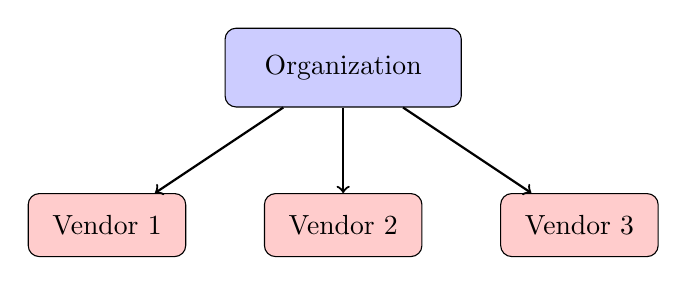
\begin{tikzpicture}
            \node[draw, rectangle, rounded corners, fill=blue!20, minimum width=3cm, minimum height=1cm] (org) at (0,0) {Organization};
            \node[draw, rectangle, rounded corners, fill=red!20, minimum width=2cm, minimum height=0.8cm] (v1) at (-3,-2) {Vendor 1};
            \node[draw, rectangle, rounded corners, fill=red!20, minimum width=2cm, minimum height=0.8cm] (v2) at (0,-2) {Vendor 2};
            \node[draw, rectangle, rounded corners, fill=red!20, minimum width=2cm, minimum height=0.8cm] (v3) at (3,-2) {Vendor 3};
            \draw[->, thick] (org) -- (v1);
            \draw[->, thick] (org) -- (v2);
            \draw[->, thick] (org) -- (v3);
        \end{tikzpicture}
    \end{center}
\end{frame}

%Slide 3
\begin{frame}
    \frametitle{Vendor Assessment: An Overview of Key Processes}
    
    \begin{itemize}
        \item \textbf{Vendor assessment} is the systematic evaluation of a third party's capabilities, security controls, and compliance posture.
        \item Assessments should be proportional to the criticality of the vendor and the sensitivity of shared data or systems.
        \item Effective vendor assessment combines multiple evaluation methods to build a comprehensive risk profile.
        \item Assessment findings inform risk mitigation strategies and ongoing monitoring requirements.
    \end{itemize}
    
    \begin{block}{Key Vendor Assessment Components}
        \begin{itemize}
            \item Security control evaluation
            \item Financial stability analysis
            \item Compliance verification
            \item Operational capability review
        \end{itemize}
    \end{block}
\end{frame}

%Slide 4
\begin{frame}
    \frametitle{Penetration Testing: Evaluating Vendor Security Defenses}
    
    \begin{itemize}
        \item \textbf{Penetration testing} involves authorized simulated attacks against a vendor's systems to identify security vulnerabilities.
        \item Tests should be conducted by qualified professionals with clearly defined parameters and objectives.
        \item Results provide valuable insights into real-world security gaps that may not be apparent through documentation review alone.
        \item Organizations should require vendors to address critical vulnerabilities identified during penetration tests.
    \end{itemize}
    
    \begin{table}
        \centering
        \begin{tabular}{ll}
            \toprule
            \textbf{Test Type} & \textbf{Focus Area} \\
            \midrule
            Black Box & External vulnerabilities without inside knowledge \\
            White Box & Comprehensive testing with full system information \\
            Web Application & Specific to web-based services and interfaces \\
            Social Engineering & Human-centered security vulnerabilities \\
            \bottomrule
        \end{tabular}
        \caption{Common Types of Penetration Tests}
    \end{table}
\end{frame}

%Slide 5
\begin{frame}
    \frametitle{Right-to-Audit Clauses: Maintaining Oversight Authority}
    
    \begin{itemize}
        \item A \textbf{right-to-audit clause} is a contractual provision granting an organization the legal authority to examine a vendor's operations and controls.
        \item These clauses establish the scope, frequency, and notification requirements for potential audits.
        \item Right-to-audit provisions are essential for verifying vendor compliance with contractual obligations and security requirements.
        \item Vendors may resist broad audit rights, necessitating careful negotiation during the contracting process.
    \end{itemize}
    
    \begin{exampleblock}{Sample Right-to-Audit Clause}
        \scriptsize
        "Customer reserves the right, upon reasonable notice, to conduct or have conducted by an independent third party, an audit of Vendor's security controls, processes, and documentation relevant to the services provided under this Agreement."
    \end{exampleblock}
\end{frame}

%Slide 6
\begin{frame}
    \frametitle{Internal Audits: What to Look for in Vendor Documentation}
    
    \begin{itemize}
        \item \textbf{Internal audits} are self-assessments conducted by vendors to evaluate their own security controls and processes.
        \item Evidence of regular internal audits demonstrates a vendor's commitment to continuous improvement and risk management.
        \item Organizations should request documentation of internal audit findings, remediation plans, and implementation timelines.
        \item The absence of internal audit processes may indicate inadequate security governance and oversight.
    \end{itemize}
    
    \begin{columns}
        \scriptsize
        \begin{column}{0.48\textwidth}
            \textbf{Effective Internal Audit Evidence:}
            \begin{itemize}
                \item Documented methodology
                \item Clear findings reports
                \item Remediation tracking
                \item Management sign-off
            \end{itemize}
        \end{column}
        \begin{column}{0.48\textwidth}
            \textbf{Red Flags:}
            \begin{itemize}
                \item Inconsistent schedules
                \item Limited scope
                \item Unresolved findings
                \item Lack of documentation
            \end{itemize}
        \end{column}
    \end{columns}
\end{frame}

%Slide 7
\begin{frame}
    \frametitle{Independent Assessments: The Value of Third-Party Verification}
    
    \begin{itemize}
        \item \textbf{Independent assessments} are evaluations conducted by qualified external parties to verify a vendor's security and compliance posture.
        \item Common examples include SOC 2 reports, ISO certifications, and industry-specific compliance audits.
        \item These assessments provide objective validation of a vendor's control environment from trusted, impartial sources.
        \item Organizations should verify the scope, timing, and qualifications of the assessors when reviewing independent assessment reports.
    \end{itemize}
    
    \begin{block}{Common Independent Assessment Types}
        \scriptsize
        \begin{tabular}{ll}
            \textbf{Assessment} & \textbf{Focus Area} \\
            \hline
            SOC 2 Type II & Security, availability, processing integrity \\
            ISO 27001 & Information security management \\
            PCI DSS & Payment card data protection \\
            HITRUST & Healthcare data security \\
        \end{tabular}
    \end{block}
\end{frame}

%Slide 8
\begin{frame}
    \frametitle{Supply Chain Analysis: Mapping Dependencies and Vulnerabilities}
    \scriptsize
    \begin{itemize}
        \item \textbf{Supply chain analysis} involves identifying and evaluating the extended network of subcontractors and suppliers that support your vendors.
        \item Organizations face indirect risks from their vendors' vendors (fourth parties) that may not be immediately apparent.
        \item Effective analysis requires mapping critical dependencies, single points of failure, and geographic concentrations.
        \item Supply chain vulnerabilities became especially evident during global disruptions like the COVID-19 pandemic.
    \end{itemize}
    
    \begin{center}
        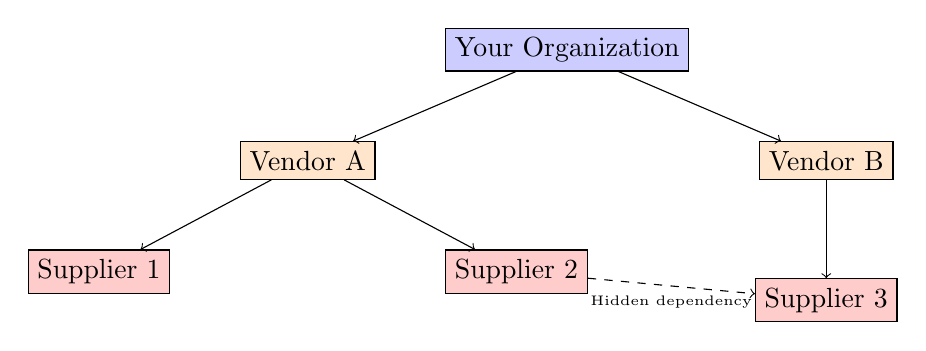
\begin{tikzpicture}[node distance=1.25cm]
            \node[draw, rectangle, fill=blue!20] (org) {Your Organization};
            \node[draw, rectangle, fill=orange!20, below left=of org] (v1) {Vendor A};
            \node[draw, rectangle, fill=orange!20, below right=of org] (v2) {Vendor B};
            \node[draw, rectangle, fill=red!20, below left=of v1] (s1) {Supplier 1};
            \node[draw, rectangle, fill=red!20, below right=of v1] (s2) {Supplier 2};
            \node[draw, rectangle, fill=red!20, below=of v2] (s3) {Supplier 3};
            
            \draw[->] (org) -- (v1);
            \draw[->] (org) -- (v2);
            \draw[->] (v1) -- (s1);
            \draw[->] (v1) -- (s2);
            \draw[->] (v2) -- (s3);
            \draw[->, dashed] (s2) -- (s3) node[midway, below, font=\tiny] {Hidden dependency};
        \end{tikzpicture}
    \end{center}
\end{frame}


%Slide 9
\begin{frame}
    \frametitle{Vendor Selection: Building a Strategic Approach}
    
    \begin{itemize}
        \item \textbf{Vendor selection} is the process of evaluating and choosing third-party providers based on predefined criteria and organizational needs.
        \item A strategic selection process balances technical capabilities, security posture, financial stability, and cost considerations.
        \item Organizations should develop a standardized selection methodology that aligns with their risk tolerance and regulatory requirements.
        \item The rigor of the selection process should be proportional to the criticality of the service and sensitivity of shared data.
    \end{itemize}
    
    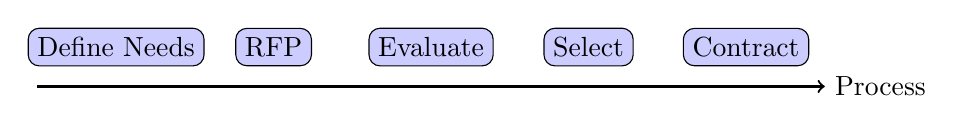
\begin{tikzpicture}
        \draw[->, thick] (0,0) -- (10,0) node[right] {Process};
        \node[draw, rectangle, rounded corners, fill=blue!20] at (1,0.5) {Define Needs};
        \node[draw, rectangle, rounded corners, fill=blue!20] at (3,0.5) {RFP};
        \node[draw, rectangle, rounded corners, fill=blue!20] at (5,0.5) {Evaluate};
        \node[draw, rectangle, rounded corners, fill=blue!20] at (7,0.5) {Select};
        \node[draw, rectangle, rounded corners, fill=blue!20] at (9,0.5) {Contract};
    \end{tikzpicture}
\end{frame}

%Slide 10
\begin{frame}
    \frametitle{Due Diligence: Investigating Before Engaging}
    
    \begin{itemize}
        \item \textbf{Due diligence} is the comprehensive investigation of a potential vendor before formalizing a business relationship.
        \item Effective due diligence examines financial stability, technical capabilities, security practices, and reputation in the market.
        \item The process identifies potential risks that may not be apparent during initial vendor presentations or marketing materials.
        \item Documentation of due diligence efforts provides evidence of reasonable care in the vendor selection process.
    \end{itemize}
    
    \begin{block}{Due Diligence Checklist}
        \scriptsize
        \begin{enumerate}
            \item Financial analysis (credit ratings, financial statements)
            \item Security assessment (policies, certifications, controls)
            \item Operational capabilities (staffing, facilities, technologies)
            \item Legal and regulatory compliance (licenses, litigation history)
            \item Business continuity planning (disaster recovery, resilience)
        \end{enumerate}
    \end{block}
\end{frame}

%Slide 11
\begin{frame}
    \frametitle{Avoiding Conflicts of Interest in Vendor Relationships}
    
    \begin{itemize}
        \item A \textbf{conflict of interest} occurs when personal or professional relationships could improperly influence vendor selection or management.
        \item Common conflicts include personal relationships with vendor staff, financial interests in vendor companies, or receiving gifts or incentives.
        \item Organizations should establish clear policies requiring disclosure of potential conflicts and recusal from decision-making when appropriate.
        \item Undisclosed conflicts of interest can lead to suboptimal vendor choices, regulatory violations, and reputational damage.
    \end{itemize}
    
    \begin{alertblock}{Warning Signs of Potential Conflicts}
        \scriptsize
        \begin{itemize}
            \item Unusual resistance to competitive bidding processes
            \item Reluctance to disclose relationships with vendors
            \item Advocating for a specific vendor despite identified deficiencies
            \item Excessive vendor entertainment or gift acceptance
        \end{itemize}
    \end{alertblock}
\end{frame}

%Slide 12
\begin{frame}
    \frametitle{Understanding Agreement Types: The Contract Landscape}
    
    \begin{itemize}
        \item \textbf{Vendor agreements} are legal documents that formalize the relationship between an organization and its third-party providers.
        \item Different agreement types serve specific purposes and vary in scope, detail, and enforceability.
        \item Well-crafted agreements clearly define expectations, responsibilities, performance metrics, and risk allocation.
        \item Understanding the appropriate agreement type for each vendor relationship is essential for effective risk management.
    \end{itemize}
    
    \begin{table}
        \scriptsize
        \centering
        \begin{tabular}{ll}
            \toprule
            \textbf{Agreement Type} & \textbf{Primary Purpose} \\
            \midrule
            Service-Level Agreement (SLA) & Define performance expectations \\
            Memorandum of Agreement (MOA) & Document mutual obligations \\
            Memorandum of Understanding (MOU) & Establish informal partnership \\
            Master Service Agreement (MSA) & Set overarching relationship terms \\
            Statement of Work (SOW) & Detail specific deliverables \\
            Non-Disclosure Agreement (NDA) & Protect confidential information \\
            Business Partners Agreement (BPA) & Structure collaborative relationships \\
            \bottomrule
        \end{tabular}
    \end{table}
\end{frame}

%Slide 13
\begin{frame}
    \frametitle{Service-Level Agreements (SLAs): Setting Performance Expectations}
    
    \begin{itemize}
        \item A \textbf{Service-Level Agreement (SLA)} is a contract that defines the expected level of service a vendor will provide.
        \item Effective SLAs include specific, measurable performance metrics such as uptime, response times, and issue resolution timeframes.
        \item SLAs should include consequences for failing to meet agreed-upon service levels, such as credits or termination rights.
        \item Regular monitoring and reporting mechanisms ensure both parties have visibility into actual performance against SLA targets.
    \end{itemize}
    
    \begin{exampleblock}{Sample SLA Metrics}
        \scriptsize
        \begin{tabular}{lll}
            \textbf{Service Aspect} & \textbf{Target} & \textbf{Penalty} \\
            \hline
            System Uptime & 99.9\% & 10\% credit for each 0.1\% below target \\
            Response Time & $<2$ seconds & 5\% credit if exceeded for $>1$ hour \\
            Support Response & 15 minutes & \$100 per hour beyond threshold \\
            Issue Resolution & 4 hours & \$500 per day beyond threshold \\
        \end{tabular}
    \end{exampleblock}
\end{frame}

%Slide 14
\begin{frame}
    \frametitle{Memorandums of Agreement (MOAs) \& Understanding (MOUs): Formal Cooperation}
    
    \begin{itemize}
        \scriptsize
        \item A \textbf{Memorandum of Agreement (MOA)} is a cooperative document that outlines specific responsibilities and commitments between parties.
        \item A \textbf{Memorandum of Understanding (MOU)} is a less formal document describing a broad concept of mutual understanding and intent to work together.
        \item MOAs are generally more detailed and binding than MOUs, though neither typically replaces comprehensive contracts for critical services.
        \item These documents are particularly useful for establishing partnerships with government entities, educational institutions, or non-profit organizations.
    \end{itemize}
    
    \begin{center}
        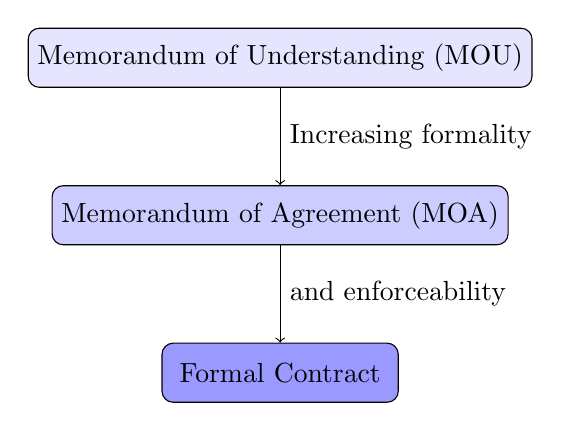
\begin{tikzpicture}
            \node (mou) at (0,0) [draw, rectangle, rounded corners, fill=blue!10, minimum width=3cm, minimum height=.75cm] {Memorandum of Understanding (MOU)};
            \node (moa) at (0,-2) [draw, rectangle, rounded corners, fill=blue!20, minimum width=3cm, minimum height=.75cm] {Memorandum of Agreement (MOA)};
            \node (contract) at (0,-4) [draw, rectangle, rounded corners, fill=blue!40, minimum width=3cm, minimum height=.75cm] {Formal Contract};
            
            \draw [->] (mou) -- (moa) node[midway, right] {Increasing formality};
            \draw [->] (moa) -- (contract) node[midway, right] {and enforceability};
        \end{tikzpicture}
    \end{center}
\end{frame}

%Slide 15
\begin{frame}
    \frametitle{Master Service Agreements (MSAs): Establishing the Relationship Foundation}
    
    \begin{itemize}
        \item A \textbf{Master Service Agreement (MSA)} is an overarching contract that establishes the fundamental terms governing the ongoing relationship between parties.
        \item MSAs typically address legal issues like liability, intellectual property, confidentiality, dispute resolution, and termination rights.
        \item The primary benefit of MSAs is efficiency, as they eliminate the need to renegotiate standard terms for each new service or project.
        \item MSAs are usually supplemented by Statements of Work or other documents that detail specific services, deliverables, and pricing.
    \end{itemize}
    
    \begin{block}{Key MSA Components}
        \scriptsize
        \begin{enumerate}
            \item \textbf{Legal Framework}: Governing law, dispute resolution, amendments
            \item \textbf{Risk Allocation}: Indemnification, liability limitations, insurance
            \item \textbf{Relationship Terms}: Duration, termination conditions, renewal processes
            \item \textbf{General Obligations}: Compliance requirements, confidentiality, security
        \end{enumerate}
    \end{block}
\end{frame}

%Slide 16
\begin{frame}
    \frametitle{Work Orders \& Statements of Work: Defining Specific Deliverables}
    
    \begin{itemize}
        \item A \textbf{Work Order (WO)} or \textbf{Statement of Work (SOW)} is a detailed document describing specific services, deliverables, timelines, and costs.
        \item These documents supplement the MSA by providing the practical details of what will be delivered in a particular engagement.
        \item An effective SOW clearly defines success criteria, milestones, acceptance procedures, and project-specific requirements.
        \item SOWs should be reviewed by technical, legal, and security stakeholders to ensure alignment with organizational needs and risk tolerance.
    \end{itemize}
    
    \begin{columns}
        \scriptsize
        \begin{column}{0.48\textwidth}
            \textbf{Essential SOW Elements:}
            \begin{itemize}
                \item Scope of work
                \item Deliverables
                \item Timeline/schedule
                \item Acceptance criteria
                \item Resources required
            \end{itemize}
        \end{column}
        \begin{column}{0.48\textwidth}
            \textbf{Common SOW Pitfalls:}
            \begin{itemize}
                \item Ambiguous requirements
                \item Undefined acceptance criteria
                \item Unrealistic timelines
                \item Missing dependencies
                \item Unclear responsibilities
            \end{itemize}
        \end{column}
    \end{columns}
\end{frame}

%Slide 17
\begin{frame}
    \frametitle{Non-Disclosure Agreements (NDAs): Protecting Sensitive Information}
    
    \begin{itemize}
        \item A \textbf{Non-Disclosure Agreement (NDA)} is a legal contract that establishes confidentiality obligations between parties.
        \item NDAs define what information is considered confidential and restrict how that information may be used or disclosed.
        \item These agreements are often executed early in vendor relationships, even before detailed discussions of sensitive business needs begin.
        \item Effective NDAs include specific provisions for data protection, permitted uses, exclusions, and remedies for unauthorized disclosure.
    \end{itemize}
    
    \begin{alertblock}{NDA Critical Elements}
        \scriptsize
        \begin{itemize}
            \item Clear definition of what constitutes "confidential information"
            \item Specific permitted uses of the confidential information
            \item Duration of confidentiality obligations (often surviving termination)
            \item Return or destruction requirements for confidential materials
            \item Meaningful remedies for breach, including injunctive relief
        \end{itemize}
    \end{alertblock}
\end{frame}

%Slide 18
\begin{frame}
    \frametitle{Business Partners Agreements (BPAs): Collaborative Frameworks}
    
    \begin{itemize}
        \small
        \item A \textbf{Business Partners Agreement (BPA)} establishes a formalized collaborative relationship between organizations with complementary capabilities.
        \item BPAs typically address revenue sharing, joint marketing, intellectual property ownership, and customer relationship management.
        \item These agreements differ from standard vendor contracts by emphasizing mutual benefit and shared responsibility rather than a pure service provider relationship.
    \end{itemize}
    
    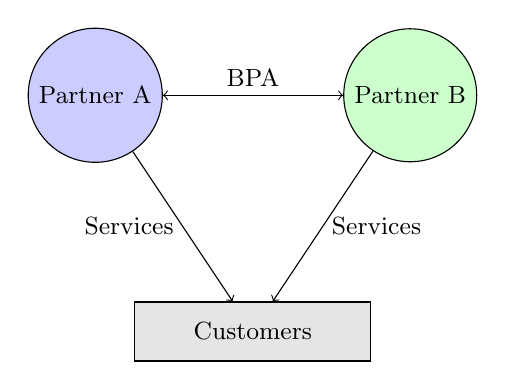
\begin{tikzpicture}
        \small
        \node (partner1) at (-2,0) [draw, circle, fill=blue!20, minimum size=1.25cm] {Partner A};
        \node (partner2) at (2,0) [draw, circle, fill=green!20, minimum size=1.25cm] {Partner B};
        \node (customers) at (0,-3) [draw, rectangle, fill=gray!20, minimum width=3cm, minimum height=.75cm] {Customers};
        
        \draw [<->] (partner1) -- (partner2) node[midway, above] {BPA};
        \draw [->] (partner1) -- (customers) node[midway, left] {Services};
        \draw [->] (partner2) -- (customers) node[midway, right] {Services};
    \end{tikzpicture}
\end{frame}

%Slide 19
\begin{frame}
    \frametitle{Ongoing Vendor Monitoring: Beyond the Contract Signing}
    
    \begin{itemize}
        \item \textbf{Vendor monitoring} is the continuous assessment of third-party performance, compliance, and risk posture throughout the relationship lifecycle.
        \item Effective monitoring includes tracking operational metrics, security posture, financial stability, and compliance with contractual obligations.
        \item The frequency and depth of monitoring activities should be proportional to the criticality of the vendor and the inherent risk of the relationship.
        \item Organizations should establish clear escalation paths for identified issues and regular executive reporting on vendor performance.
    \end{itemize}
    
    \begin{block}{Vendor Monitoring Framework}
        \scriptsize
        \begin{tabular}{ll}
            \textbf{Monitoring Type} & \textbf{Frequency} \\
            \hline
            Performance Review & Monthly \\
            Security Assessment & Quarterly \\
            Financial Health Check & Annually \\
            Comprehensive Reassessment & Every 1-3 years \\
            Continuous Monitoring & Real-time alerts \\
        \end{tabular}
    \end{block}
\end{frame}

%Slide 20
\begin{frame}
    \frametitle{Developing Effective Assessment Questionnaires}
    
    \begin{itemize}
        \item \textbf{Assessment questionnaires} are structured tools used to collect information about a vendor's controls, capabilities, and practices.
        \item Effective questionnaires include a mix of yes/no, multiple-choice, and open-ended questions with requests for supporting evidence.
        \item Questions should be tailored to the specific service being provided and the risks inherent in that service.
        \item Industry standard questionnaires like the Standardized Information Gathering (SIG) or Vendor Security Alliance (VSA) provide comprehensive starting points.
    \end{itemize}
    
    \begin{columns}
        \scriptsize
        \begin{column}{0.48\textwidth}
            \textbf{Questionnaire Best Practices:}
            \begin{itemize}
                \item Right-size to vendor criticality
                \item Focus on evidence, not just assertions
                \item Include verification methods
                \item Evaluate answers holistically
            \end{itemize}
        \end{column}
        \begin{column}{0.48\textwidth}
            \textbf{Key Assessment Areas:}
            \begin{itemize}
                \item Information security
                \item Business continuity
                \item Privacy practices
                \item Regulatory compliance
                \item Subcontractor management
            \end{itemize}
        \end{column}
    \end{columns}
\end{frame}

%Slide 21
\begin{frame}
    \frametitle{Rules of Engagement: Setting Clear Boundaries and Procedures}
    
    \begin{itemize}
        \item \textbf{Rules of engagement} establish the parameters and protocols for interactions between an organization and its vendors.
        \item These rules define authorized activities, communication channels, escalation procedures, and access limitations.
        \item Clear rules of engagement are particularly critical for security testing, system access, and data handling activities.
        \item Documented and agreed-upon rules protect both parties by establishing shared expectations and limiting liability.
    \end{itemize}
    
    \begin{exampleblock}{Sample Rules of Engagement for Security Testing}
        \scriptsize
        \begin{itemize}
            \item Testing window: July 15-20, 2025, between 10:00 PM and 4:00 AM EST
            \item Test targets: Web applications at domains xyz.com and admin.xyz.com only
            \item Prohibited actions: Denial of service attacks, social engineering, physical security testing
            \item Emergency contacts: Jane Smith (555-123-4567), John Doe (555-789-0123)
            \item Test termination authority: CISO or Security Operations Manager
        \end{itemize}
    \end{exampleblock}
\end{frame}

%Slide 22
\begin{frame}
    \frametitle{Case Study: Third-Party Risk Management in Action}
    
    \begin{itemize}
        \item A financial institution discovered a critical vulnerability in a third-party payment processing system through routine security testing.
        \item The vulnerability could have exposed customer financial data and violated multiple regulatory requirements if exploited.
        \item The institution invoked their right-to-audit clause and conducted an emergency assessment of the vendor's security controls.
        \item A remediation plan was developed with clear timelines, verification requirements, and consequences for non-compliance.
    \end{itemize}
    
    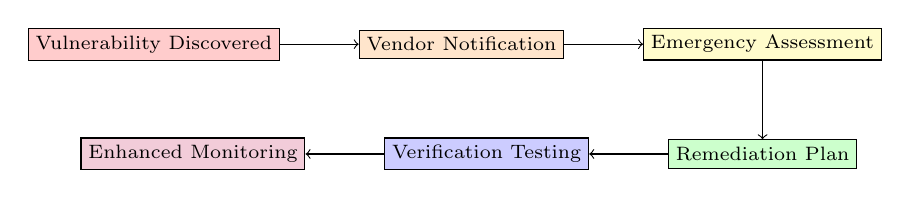
\begin{tikzpicture}[node distance=1.0cm]
        \scriptsize
        \node[draw, rectangle, fill=red!20] (issue) {Vulnerability Discovered};
        \node[draw, rectangle, fill=orange!20, right=of issue] (notify) {Vendor Notification};
        \node[draw, rectangle, fill=yellow!20, right=of notify] (assess) {Emergency Assessment};
        \node[draw, rectangle, fill=green!20, below=of assess] (plan) {Remediation Plan};
        \node[draw, rectangle, fill=blue!20, left=of plan] (verify) {Verification Testing};
        \node[draw, rectangle, fill=purple!20, left=of verify] (monitor) {Enhanced Monitoring};
        
        \draw[->] (issue) -- (notify);
        \draw[->] (notify) -- (assess);
        \draw[->] (assess) -- (plan);
        \draw[->] (plan) -- (verify);
        \draw[->] (verify) -- (monitor);
    \end{tikzpicture}
\end{frame}

%Slide 23
\begin{frame}
    \frametitle{Best Practices: Building an Effective Vendor Management Program}
    
    \begin{itemize}
        \item Establish a formal \textbf{vendor risk management program} with defined roles, responsibilities, and governance structures.
        \item Implement a \textbf{risk-based approach} that allocates resources according to vendor criticality and the sensitivity of shared data or systems.
        \item Maintain a comprehensive \textbf{vendor inventory} with risk classifications, relationship owners, and contract information.
        \item Develop \textbf{standardized processes} for vendor selection, contracting, onboarding, monitoring, and offboarding.
    \end{itemize}
    
    \begin{block}{Program Maturity Model}
        \scriptsize
        \begin{tabular}{lll}
            \textbf{Level} & \textbf{Characteristics} & \textbf{Focus} \\
            \hline
            Initial & Reactive, ad-hoc & Individual vendors \\
            Developing & Basic processes & Critical vendors \\
            Established & Consistent approach & All significant vendors \\
            Advanced & Proactive management & Entire vendor ecosystem \\
            Optimized & Continuous improvement & Strategic partnerships \\
        \end{tabular}
    \end{block}
\end{frame}

%Slide 24
\begin{frame}
    \frametitle{Conclusion: Integrating Third-Party Risk into Organizational Strategy}
    
    \begin{itemize}
        \item Effective third-party risk management is not just a compliance exercise but a critical component of organizational resilience.
        \item Organizations should view vendors as extensions of their own operations, applying appropriate oversight proportional to the risk exposure.
        \item A strategic approach balances risk mitigation with business enablement, recognizing that vendor relationships are essential for growth and innovation.
        \item As organizations increasingly rely on complex networks of third parties, mature vendor management becomes a competitive advantage.
    \end{itemize}
    
    \begin{alertblock}{Key Takeaways}
        \scriptsize
        \begin{enumerate}
            \item Adopt a risk-based approach to vendor management
            \item Establish clear contractual protections and monitoring mechanisms
            \item Maintain comprehensive documentation of assessment and monitoring activities
            \item Develop incident response plans that include vendor-related scenarios
            \item Regularly review and update your vendor management program as threats evolve
        \end{enumerate}
    \end{alertblock}
\end{frame}


\end{document}